% \begin{table}
% \begin{tabular}{|l|cc|}
% \hline
% Category & $N_{\textrm{events}}$ & (\%) \\
% \hline
% Lepton fiducial & 67.5 & 0.56 \\
% Lepton jet overlap & 50.6 & 0.42 \\
% Lepton non-prompt & 10.9 & 0.09 \\
% $b$-jet fiducial & 245.8 & 2.05 \\
% $b$-jet other & 123.4 & 1.03 \\
% \hline
% Fakes total & 498.2 & 4.15 \\
% \hline \hline
% Passes reco and truth selection & 11499.0 & 95.85 \\
% \hline
% \end{tabular}
% \captionsetup{singlelinecheck=off}
% \caption[]{Number of events passing selection requirements at the reconstruction level in \pow+\py \ttbar simulation. The subset of events that pass at reconstruction but not particle level are broken down into contributions from:
% \begin{center}
% \begin{itemize}
% \item[\textbf{Lepton fiducial:}] dressed truth $e$ or $\mu$ fails the fiducial $p_{T}$ or $\eta$ cuts
% \item[\textbf{Lepton jet overlap:}] dressed truth $e$ or $\mu$  overlaps with a truth jet
% \item[\textbf{Lepton non-prompt:}] truth $e$ or $\mu$ leptons from a hadron or other background
% \item[\textbf{$b$-jet fiducial:}] truth $b$-jet fails the fiducial $p_{T}$ or $\eta$ cuts
% \item[\textbf{$b$-jet other:}] truth jet not matched to $B$ hadron, meaning that the reconstructed $b$-jet was mistagged. Also includes small number of cases where the two reconstructed $b$-jets are matched to a single truth jet or one of the two reconstructed $b$-jets does not have a truth match.
% \end{itemize}
% \end{center}
% }

% \label{t:fakes}
% \end{table}

This appendix compares the kinematic distributions for the reconstructed objects in events that pass both the
the reconstruction level and truth let event selection to those that pass the reconstruction selection 
but fail the truth event selection.   Failed events are divided into categories based on which object fails
the truth selection.  The selection cuts are applied in the order given in the figure legends.  Events that
fail one cut are not tested against subsequent cuts.  A subset of the figures from this section are also presented
in Figure~\ref{fig:reconottruth}. 

Figure~\ref{fig:fakeemu}
shows the \pt\ and $\eta$ distributions of the reconstructed leptons.   The \pt, $\eta$ and MV1 of the reconstructed
$b$-jets are provided in Figure~\ref{fig:fakebjet}. The extra jet multiplicity and the \pt\ spectrum for extra
jets of rank 1 through 5 are given in Figure~\ref{fig:fakejetpt}.

\begin{figure}
\centering
\begin{subfigure}[]{0.45\textwidth}
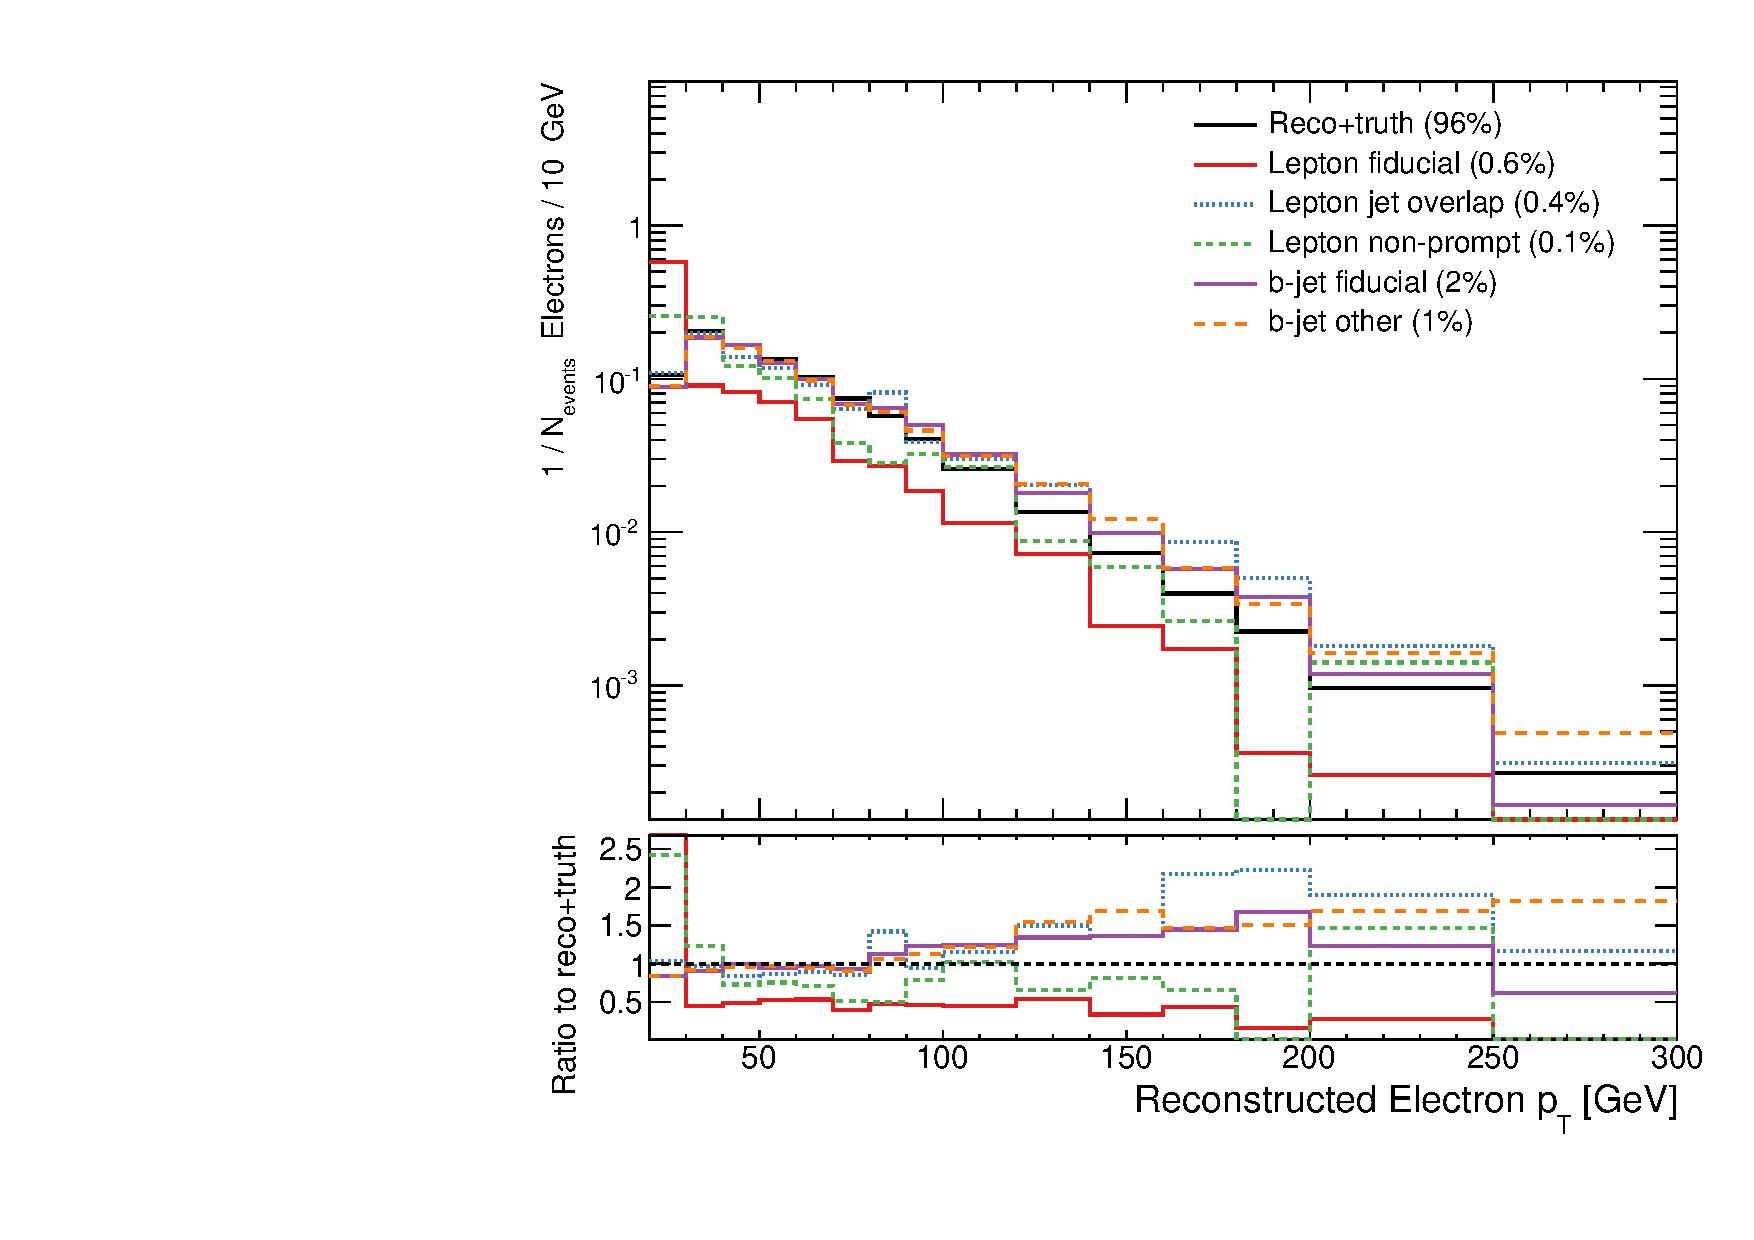
\includegraphics[width=\textwidth]{fig/RecoNotTruth/ElecPt.pdf}
\end{subfigure}
\begin{subfigure}[]{0.45\textwidth}
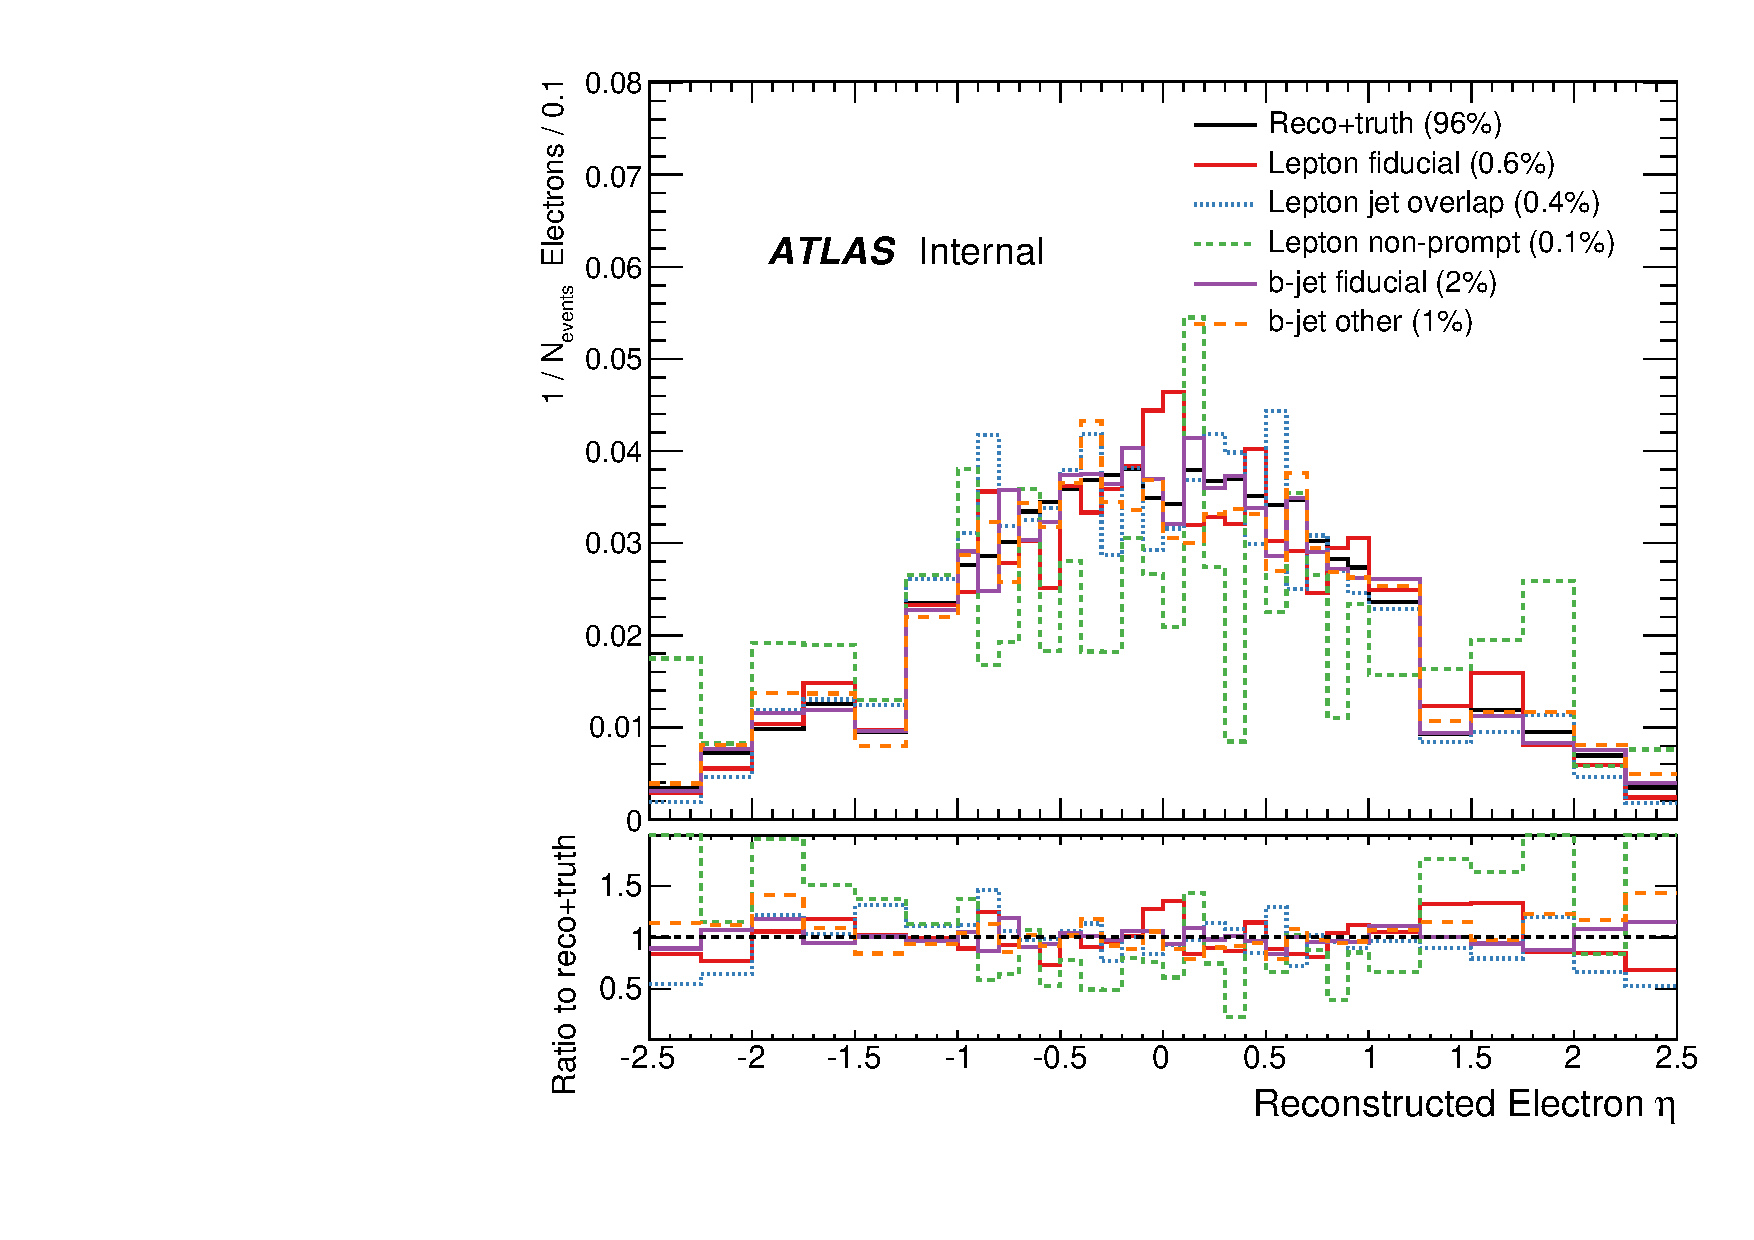
\includegraphics[width=\textwidth]{fig/RecoNotTruth/ElecEta.pdf}
\end{subfigure}
\\
\begin{subfigure}[]{0.45\textwidth}
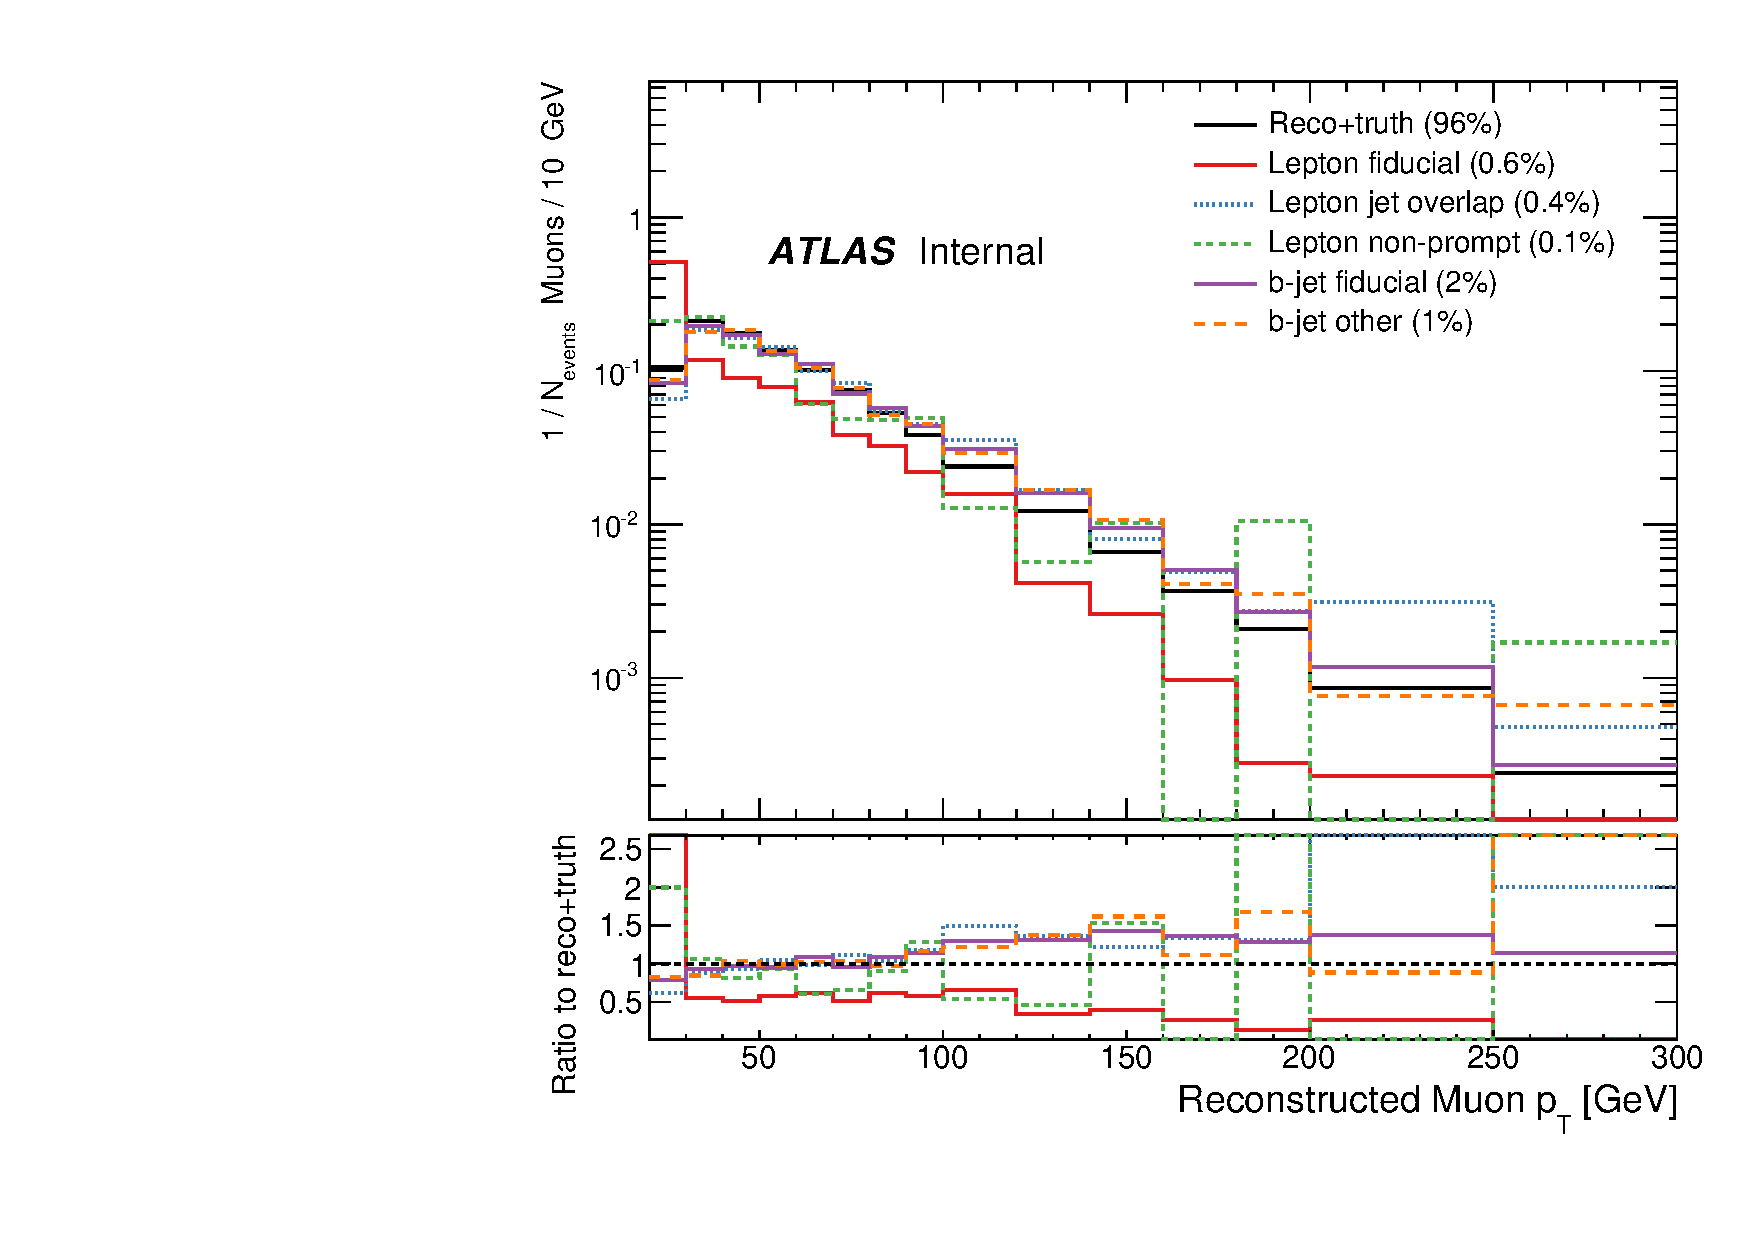
\includegraphics[width=\textwidth]{fig/RecoNotTruth/MuPt.pdf}
\end{subfigure}
\begin{subfigure}[]{0.45\textwidth}
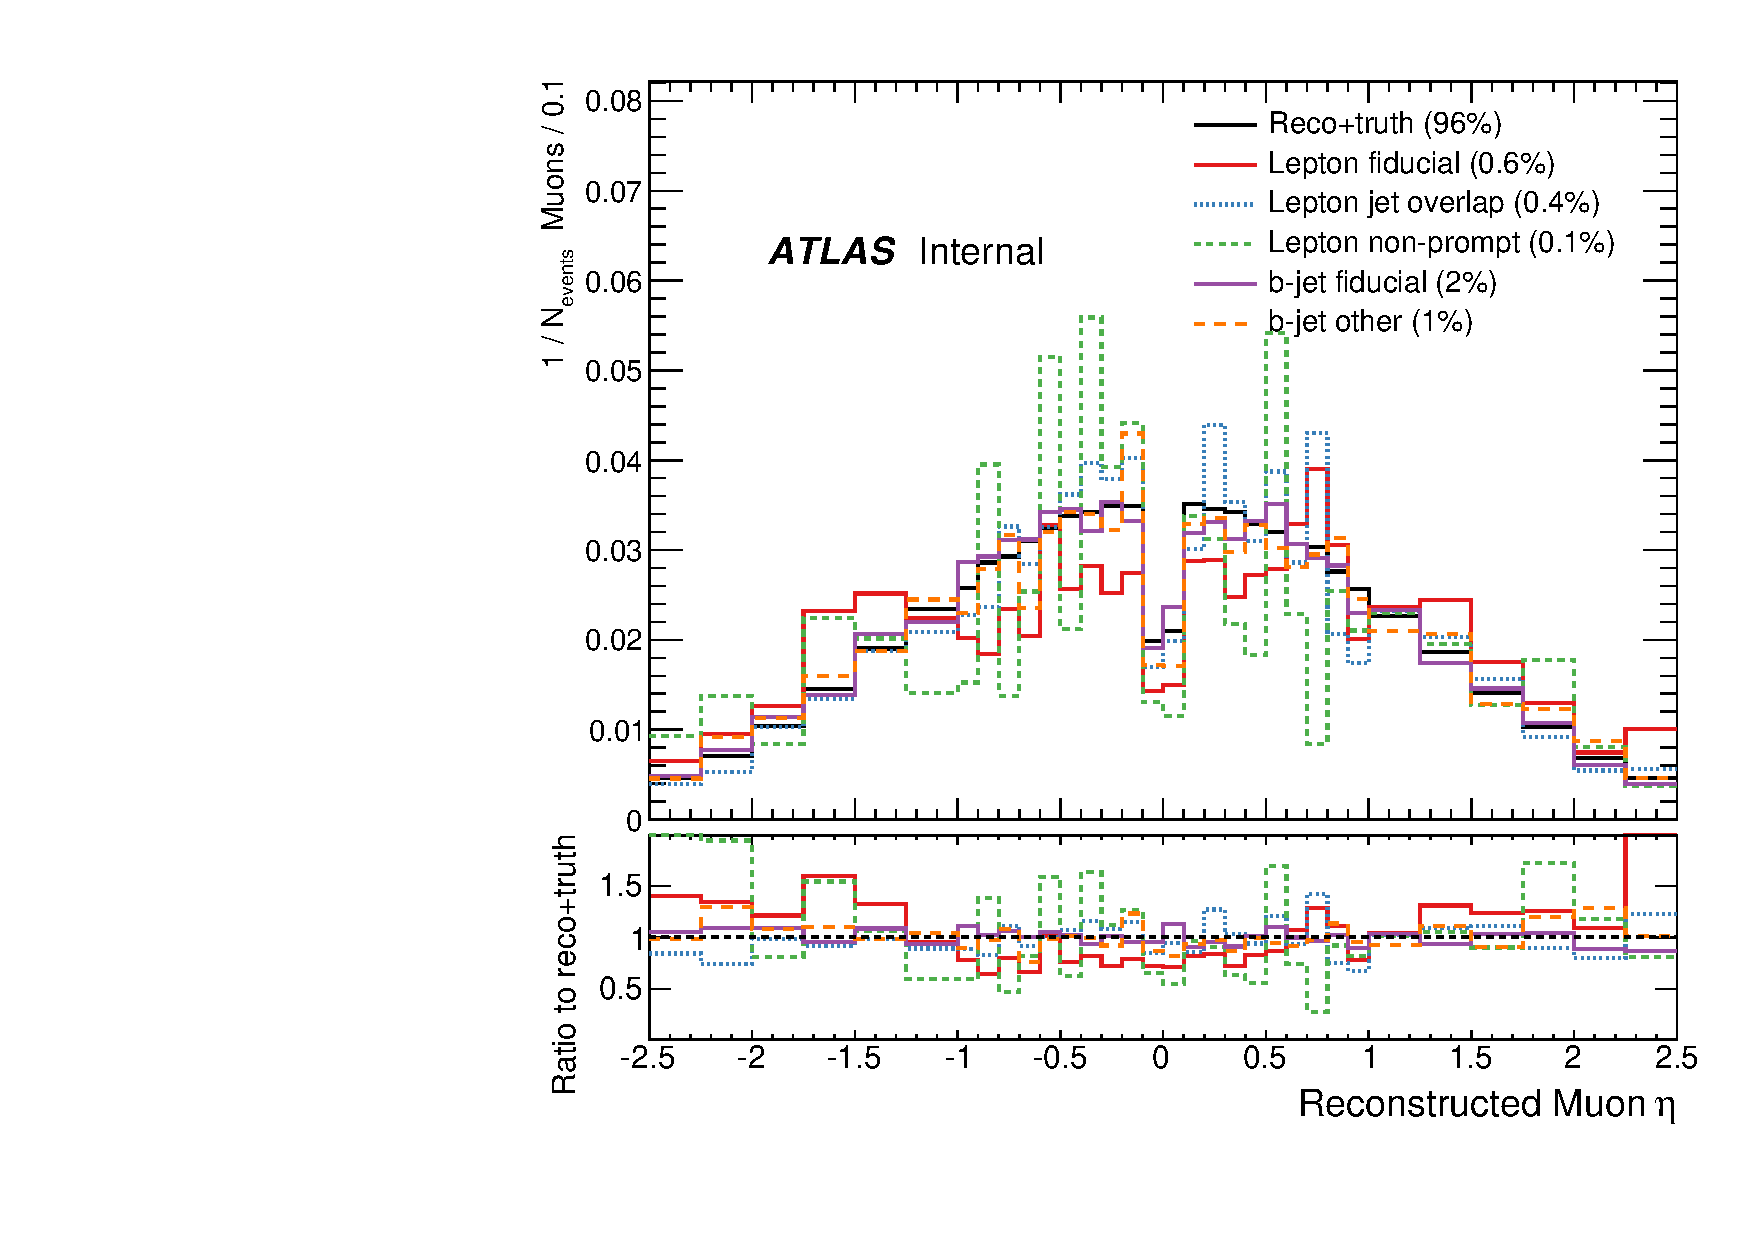
\includegraphics[width=\textwidth]{fig/RecoNotTruth/MuEta.pdf}
\end{subfigure}
\caption{Distributions of the $e$ and $\mu$ \pt and $\eta$ for events in different truth categories. Each distribution is normalized by the number of events falling in that category. Events were simulated with \pow+\py \ttbar.}
\label{fig:fakeemu}
\end{figure}

\begin{figure}
\centering
\begin{subfigure}[]{0.45\textwidth}
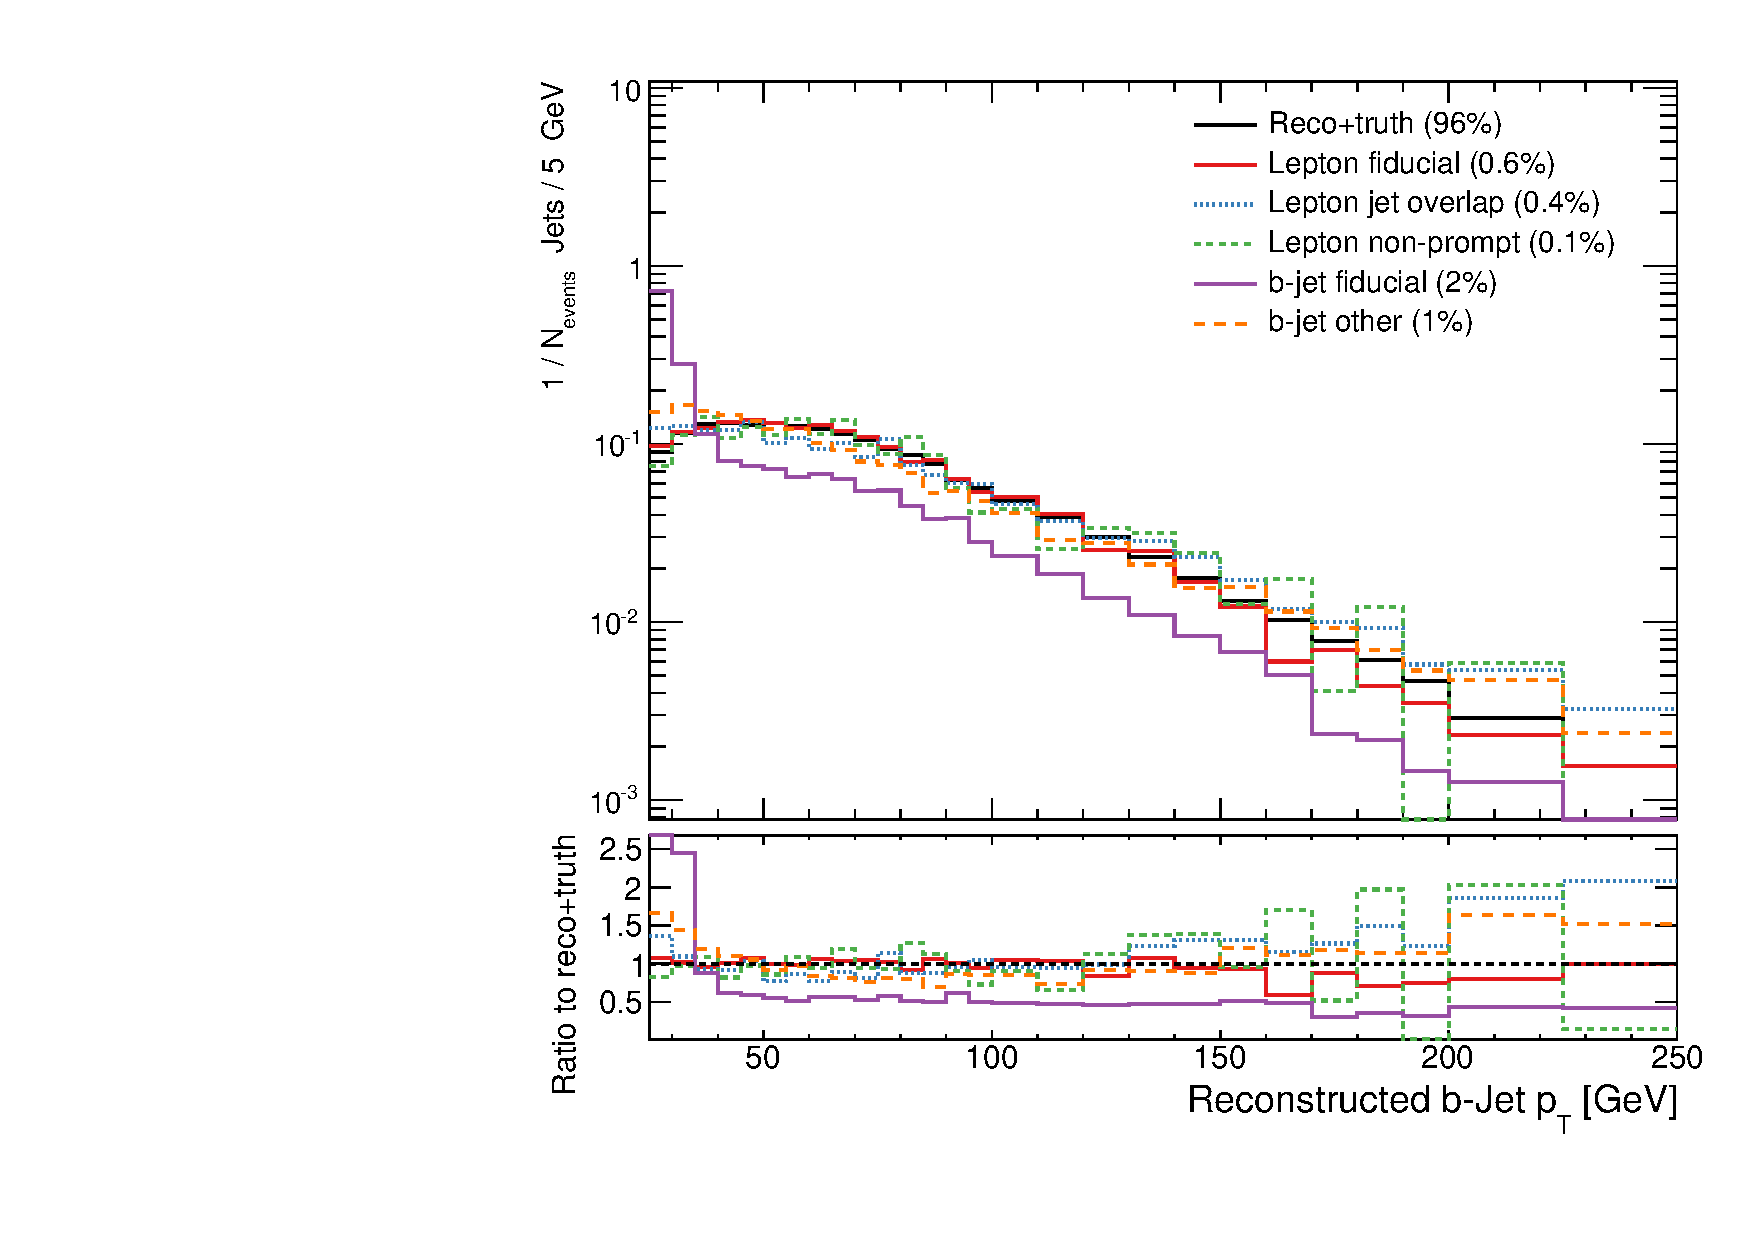
\includegraphics[width=\textwidth]{fig/RecoNotTruth/BJetPt.pdf}
\end{subfigure}
\begin{subfigure}[]{0.45\textwidth}
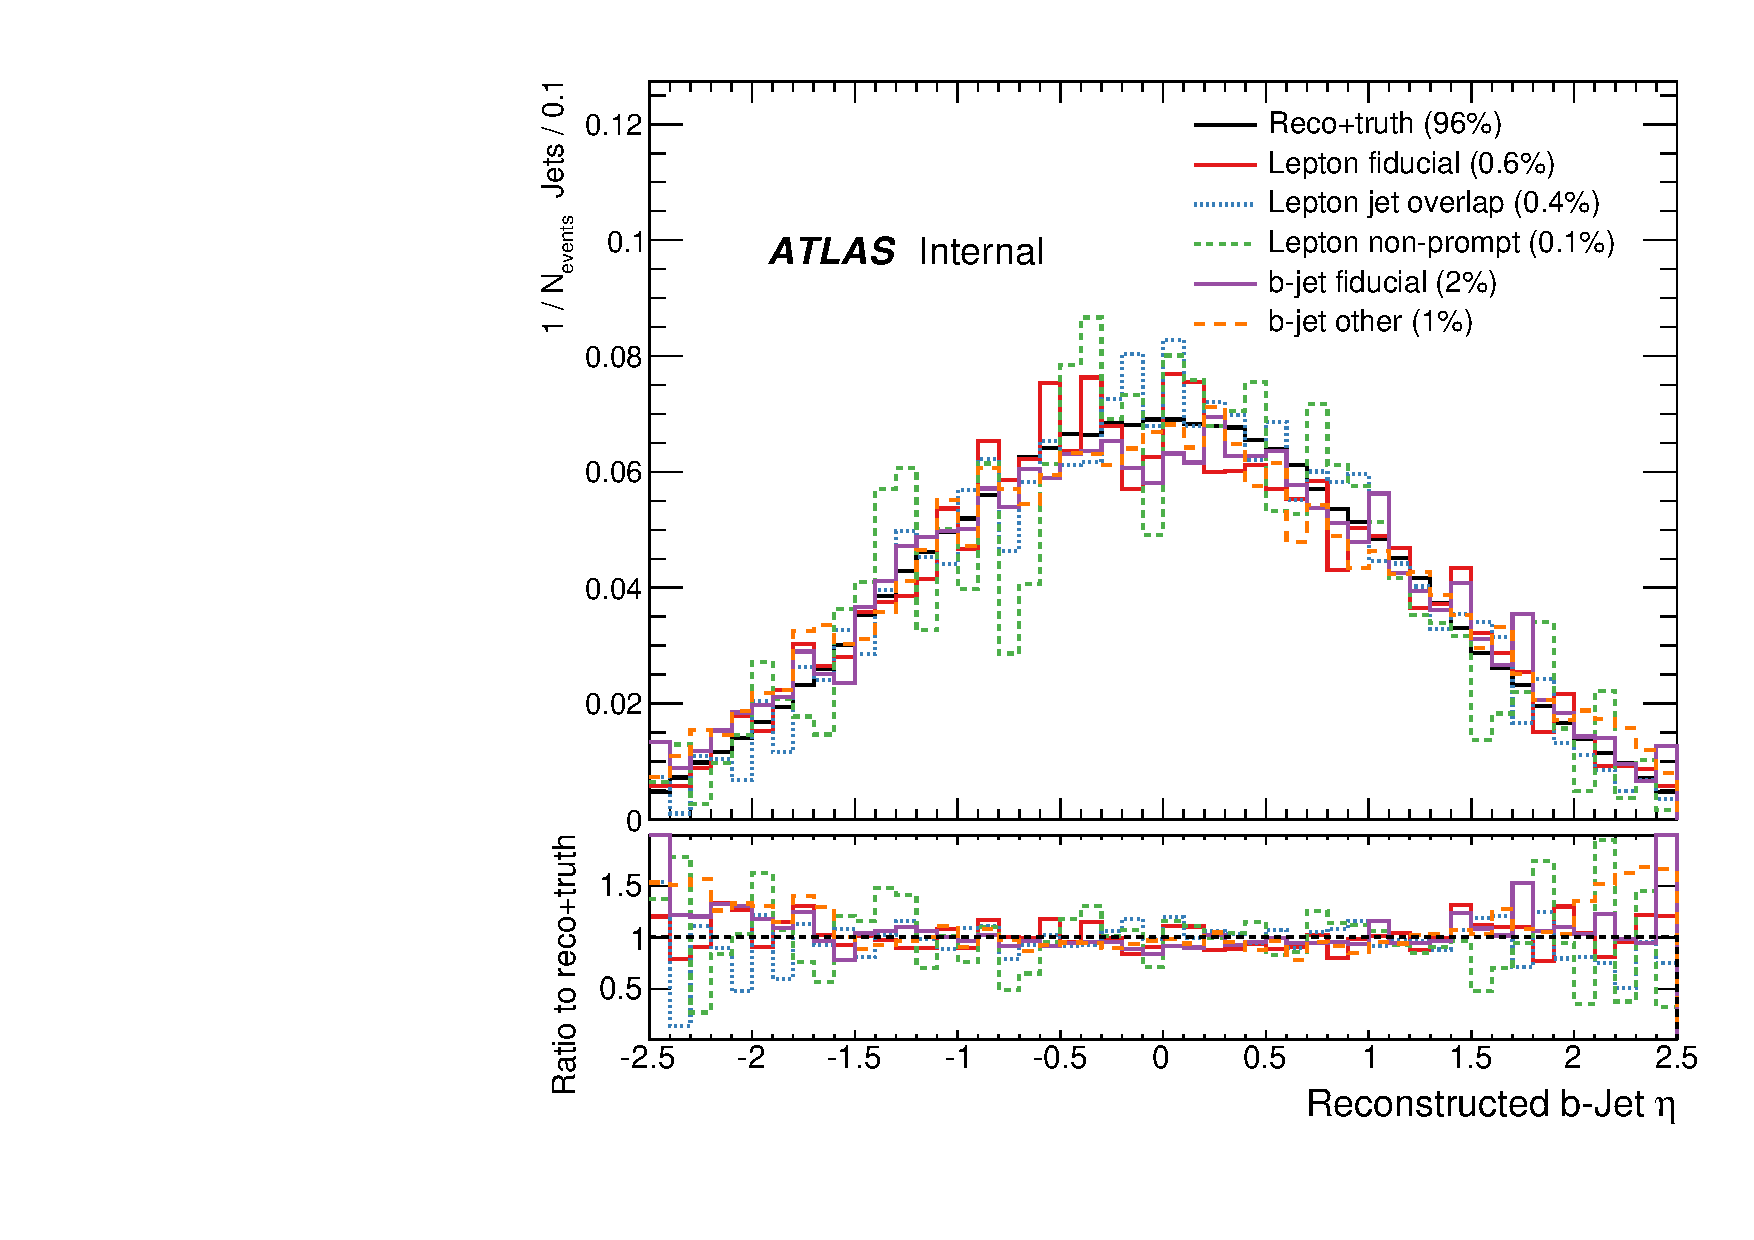
\includegraphics[width=\textwidth]{fig/RecoNotTruth/BJetEta.pdf}
\end{subfigure}
\\
\begin{subfigure}[]{0.45\textwidth}
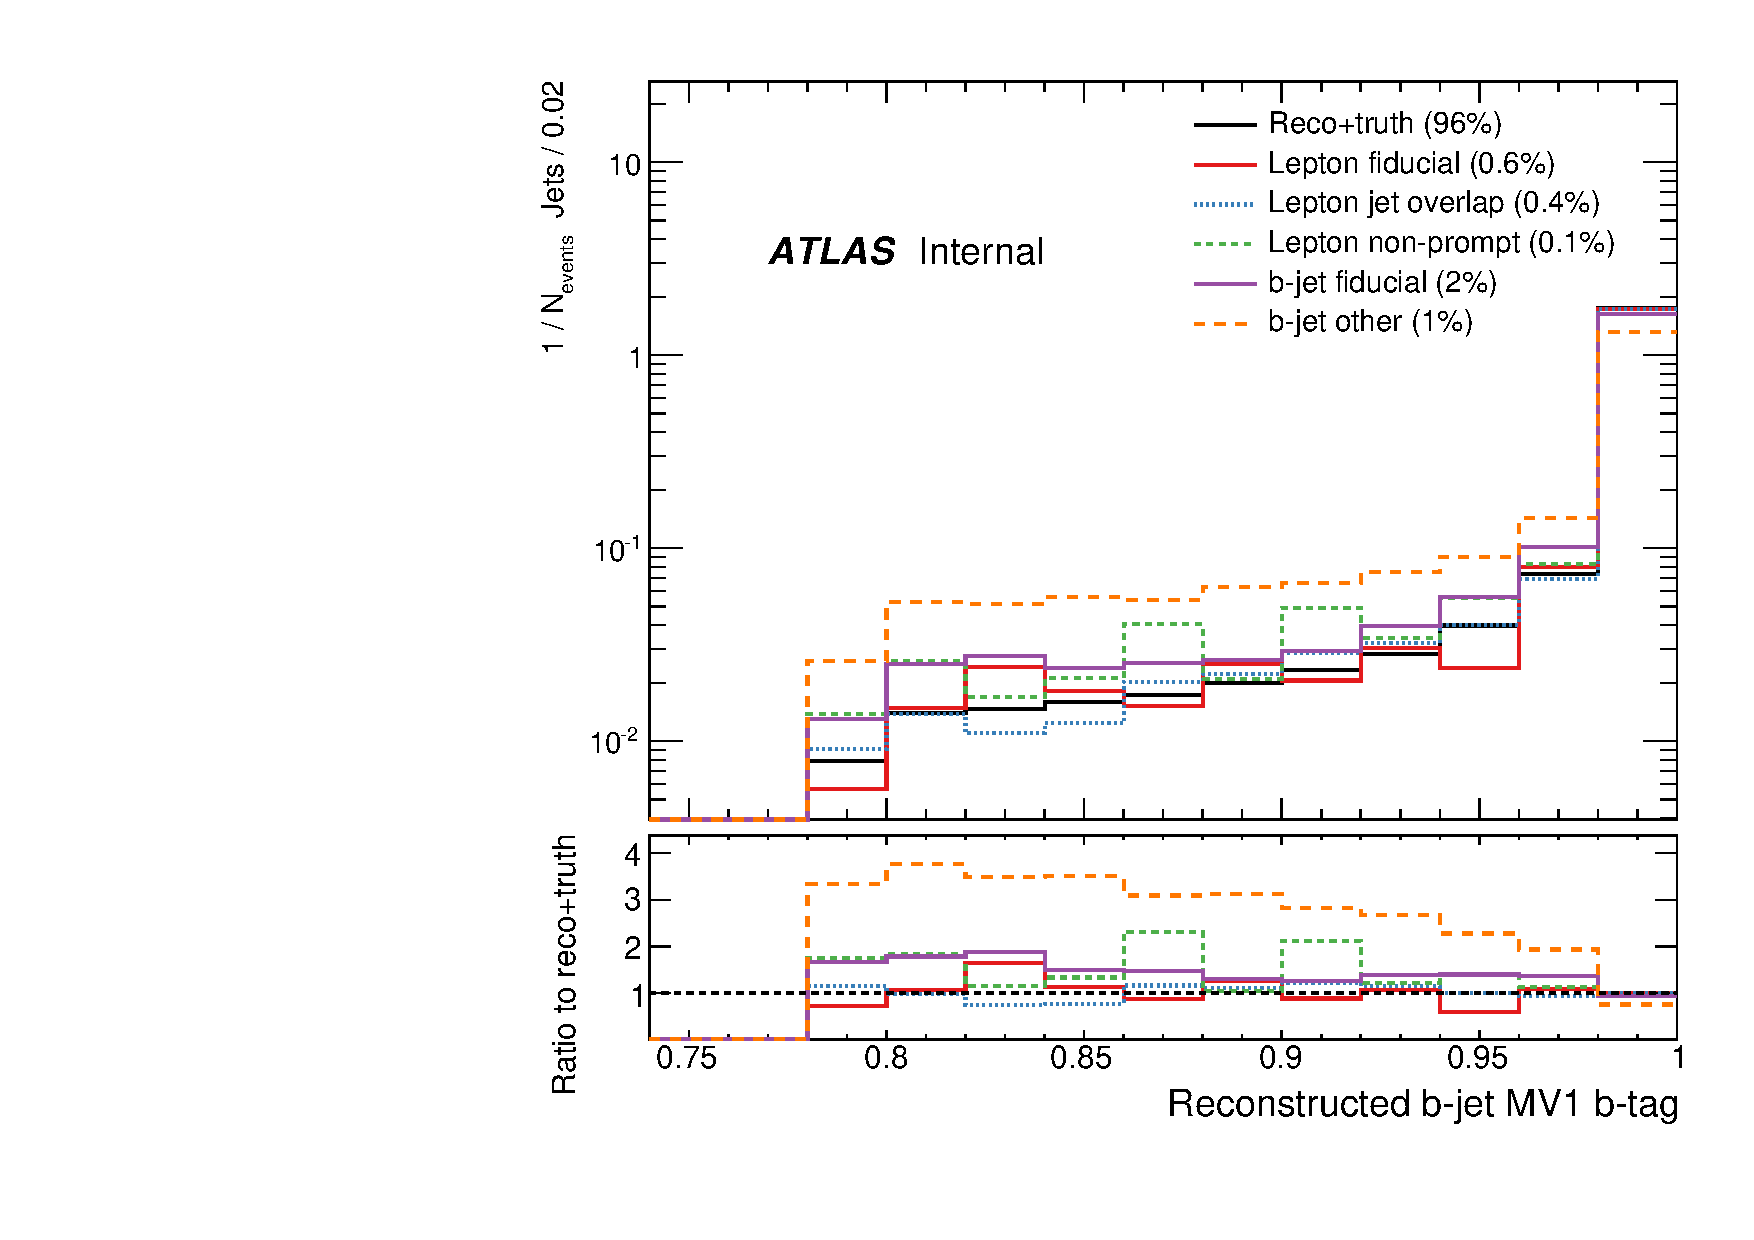
\includegraphics[width=\textwidth]{fig/RecoNotTruth/BJetMV1.pdf}
\end{subfigure}
\caption{Distributions of the $b$-jet \pt, $\eta$, and MV1 for events in different truth categories. Each distribution is normalized by the number of events falling in that category. }
\label{fig:fakebjet}
\end{figure}

\begin{figure}
\centering
\begin{subfigure}[]{0.3\textwidth}
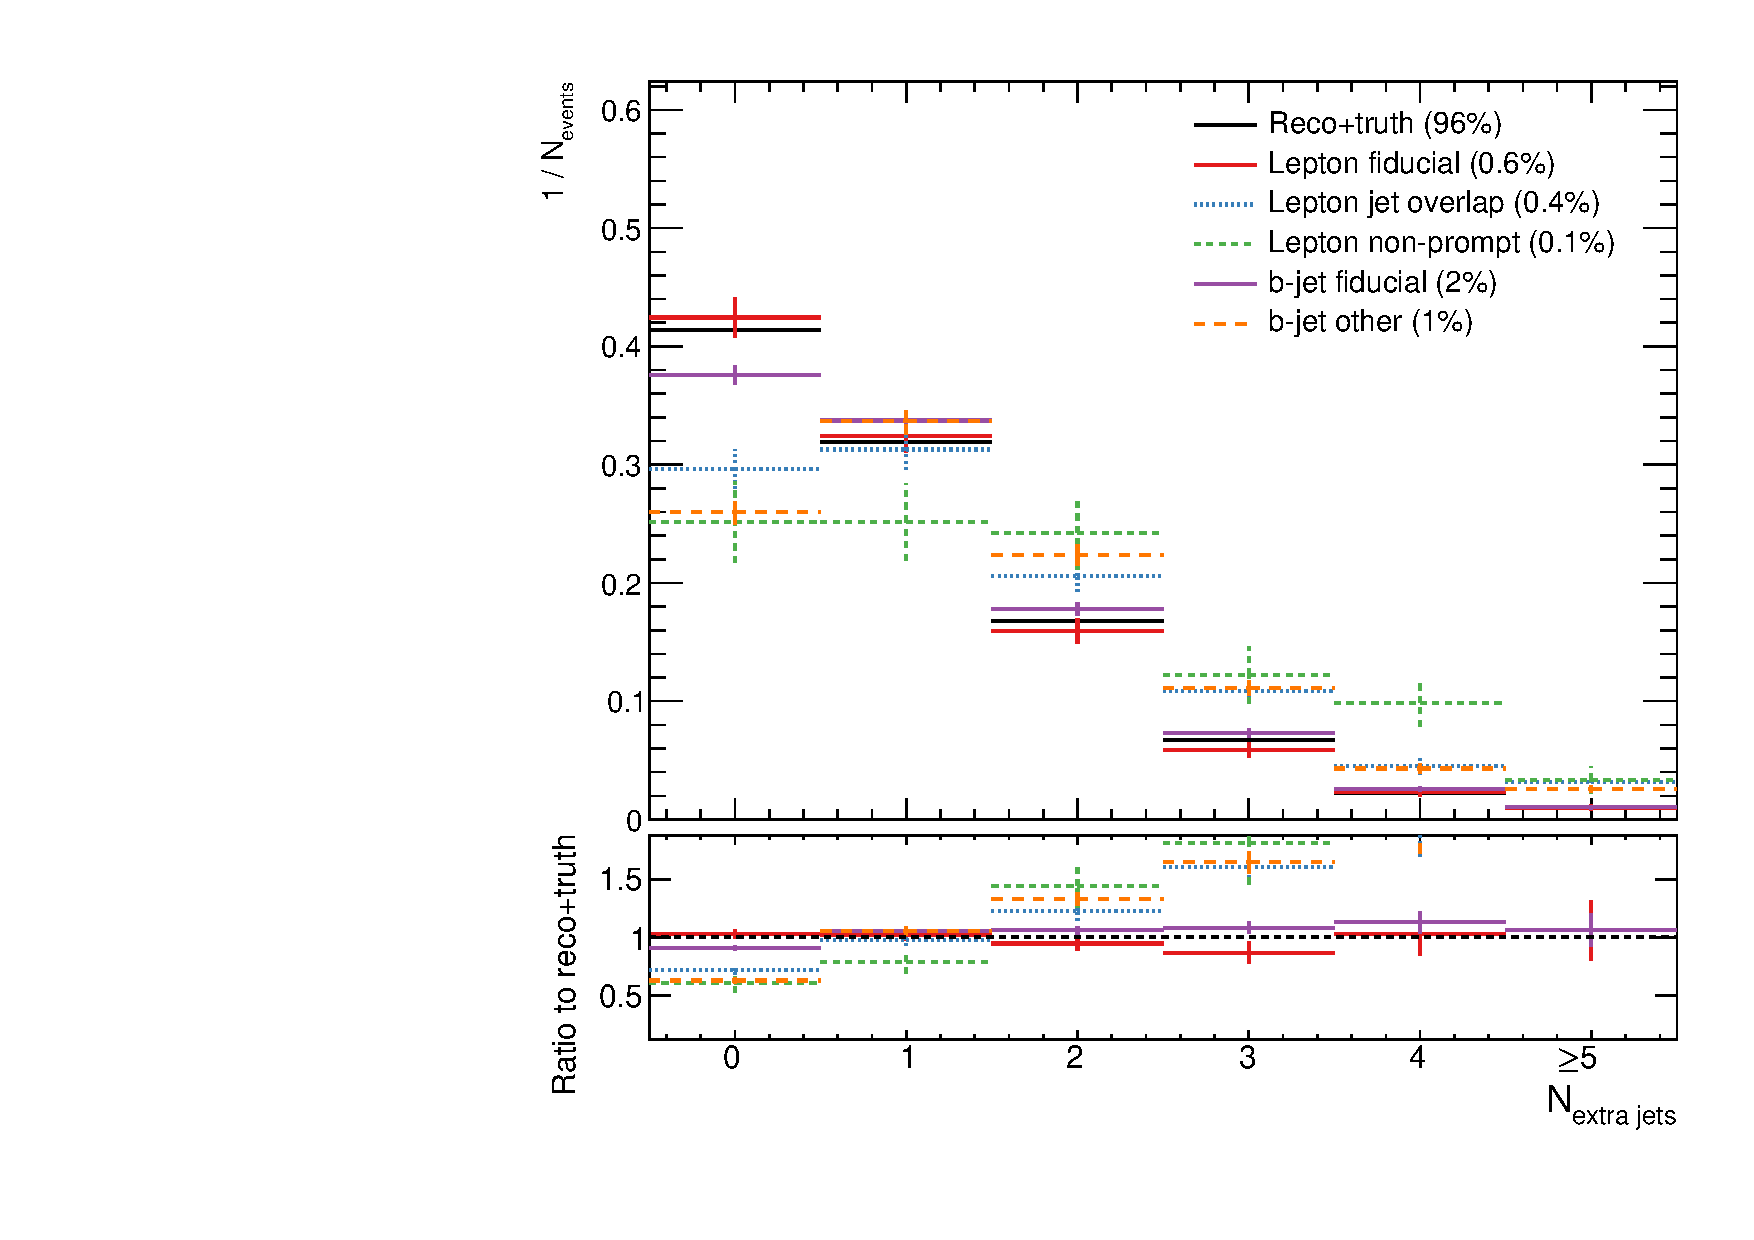
\includegraphics[width=\textwidth]{fig/RecoNotTruth/NJets.pdf}
\end{subfigure}
~
\begin{subfigure}[]{0.3\textwidth}
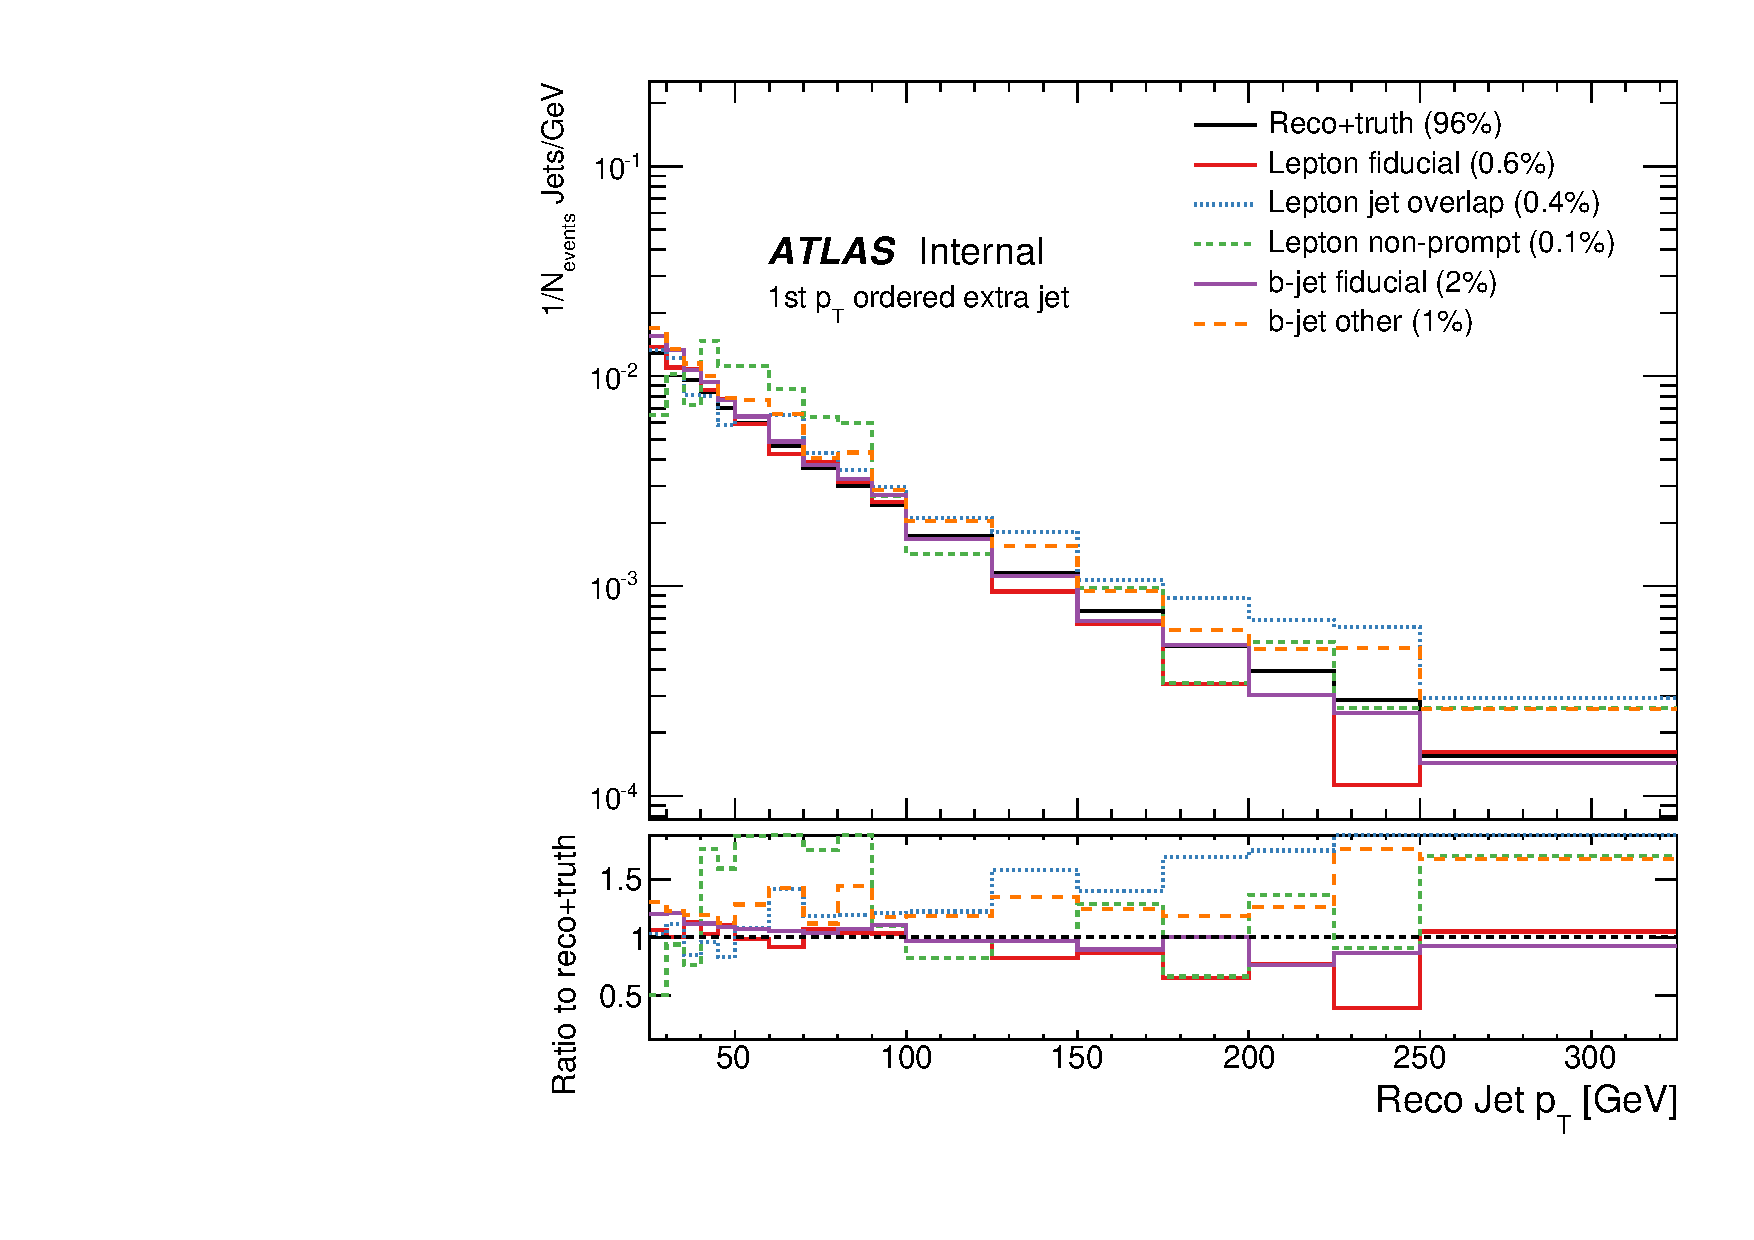
\includegraphics[width=\textwidth]{fig/RecoNotTruth/RecoPtJet0.pdf}
\end{subfigure}
~
\begin{subfigure}[]{0.3\textwidth}
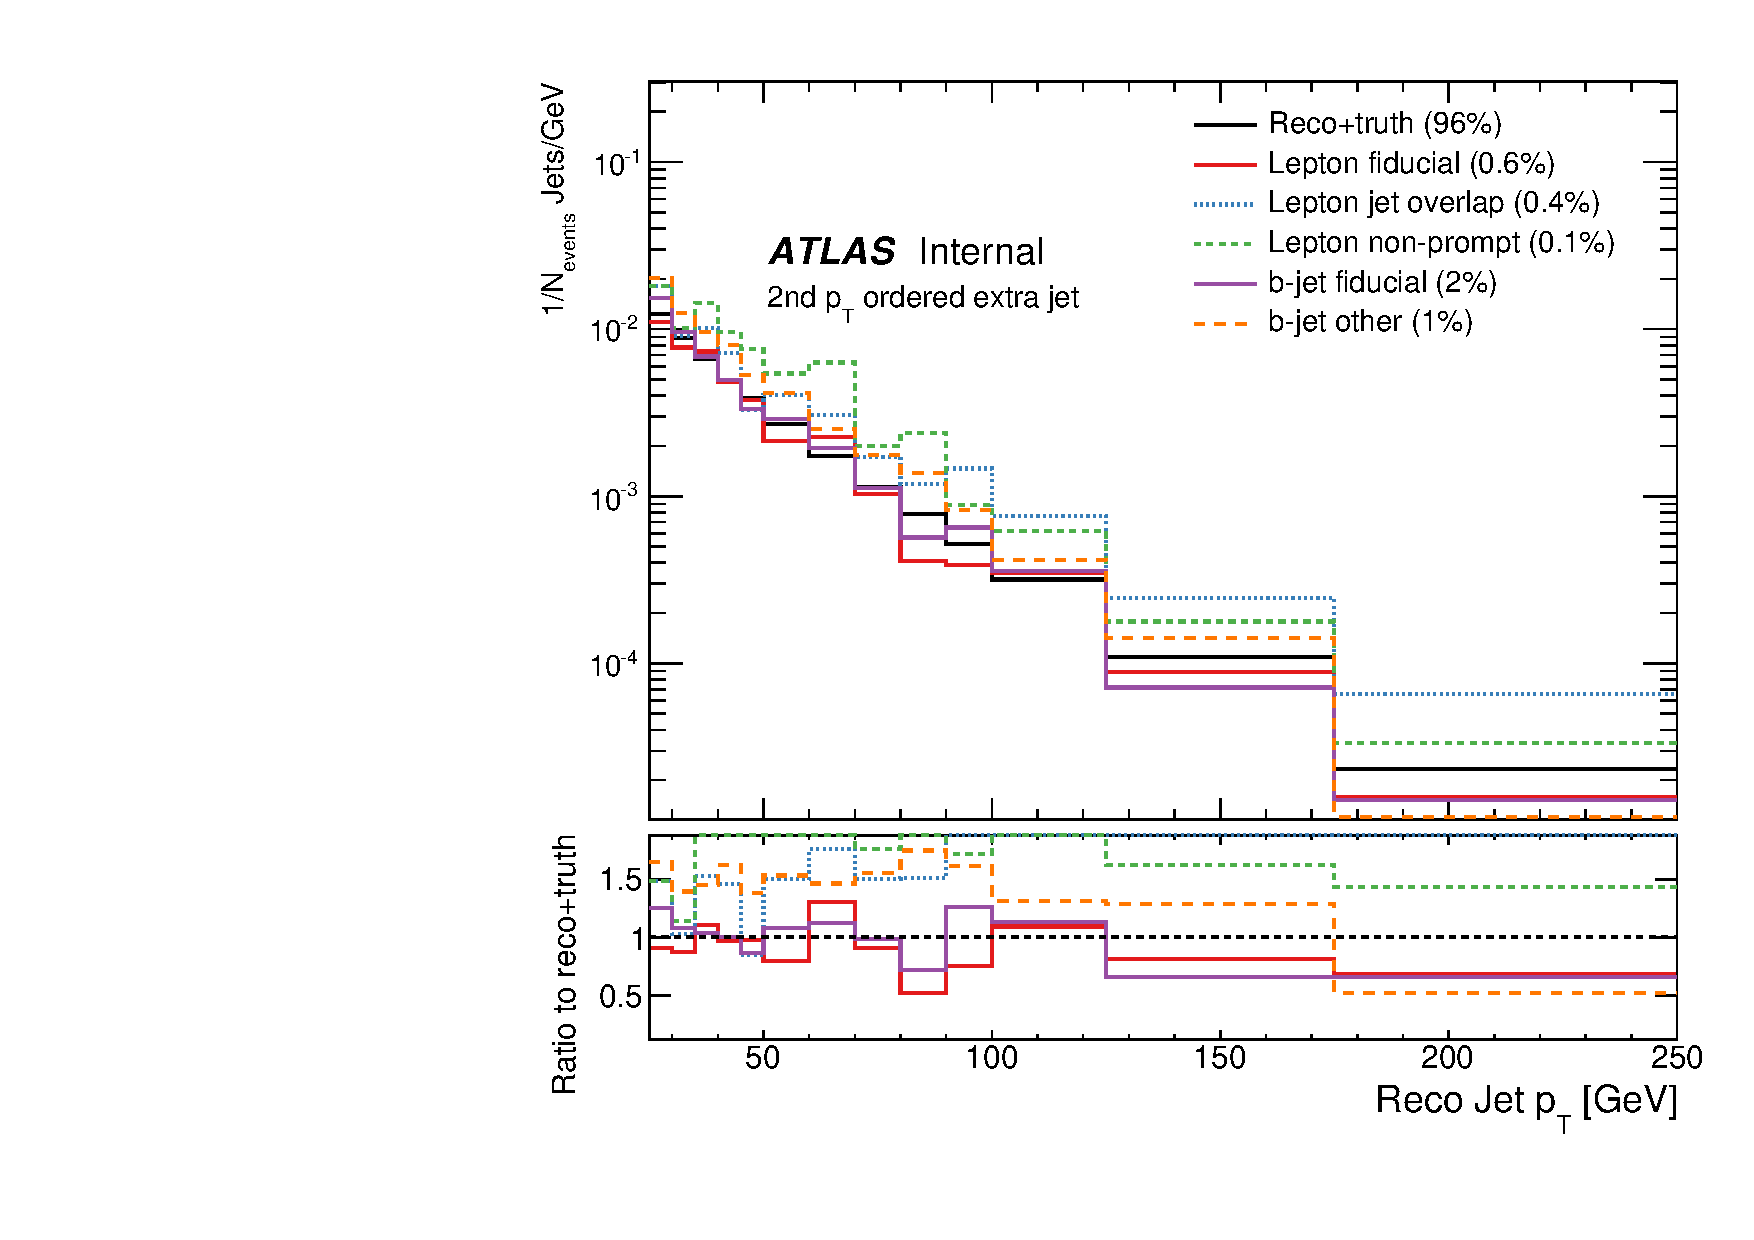
\includegraphics[width=\textwidth]{fig/RecoNotTruth/RecoPtJet1.pdf}
\end{subfigure}
~
\begin{subfigure}[]{0.3\textwidth}
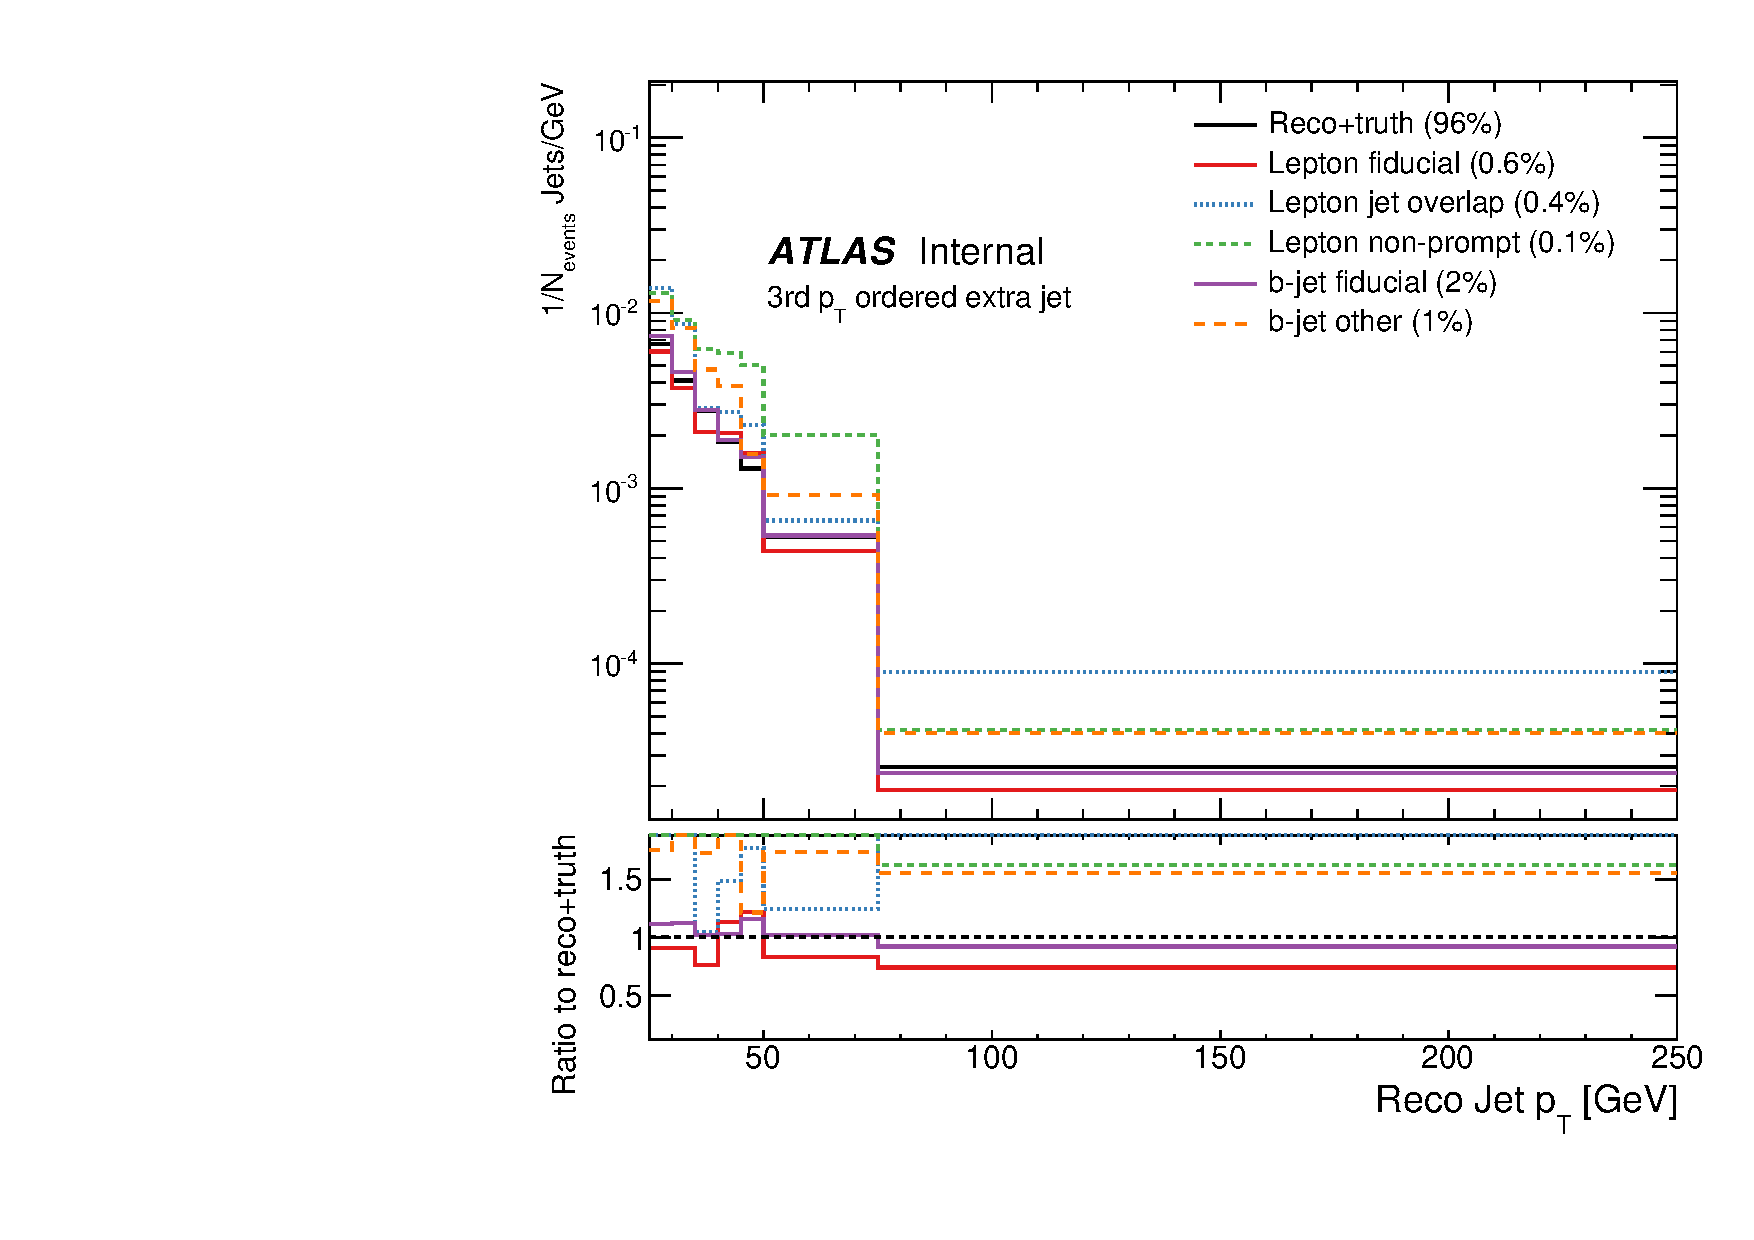
\includegraphics[width=\textwidth]{fig/RecoNotTruth/RecoPtJet2.pdf}
\end{subfigure}
~
\begin{subfigure}[]{0.3\textwidth}
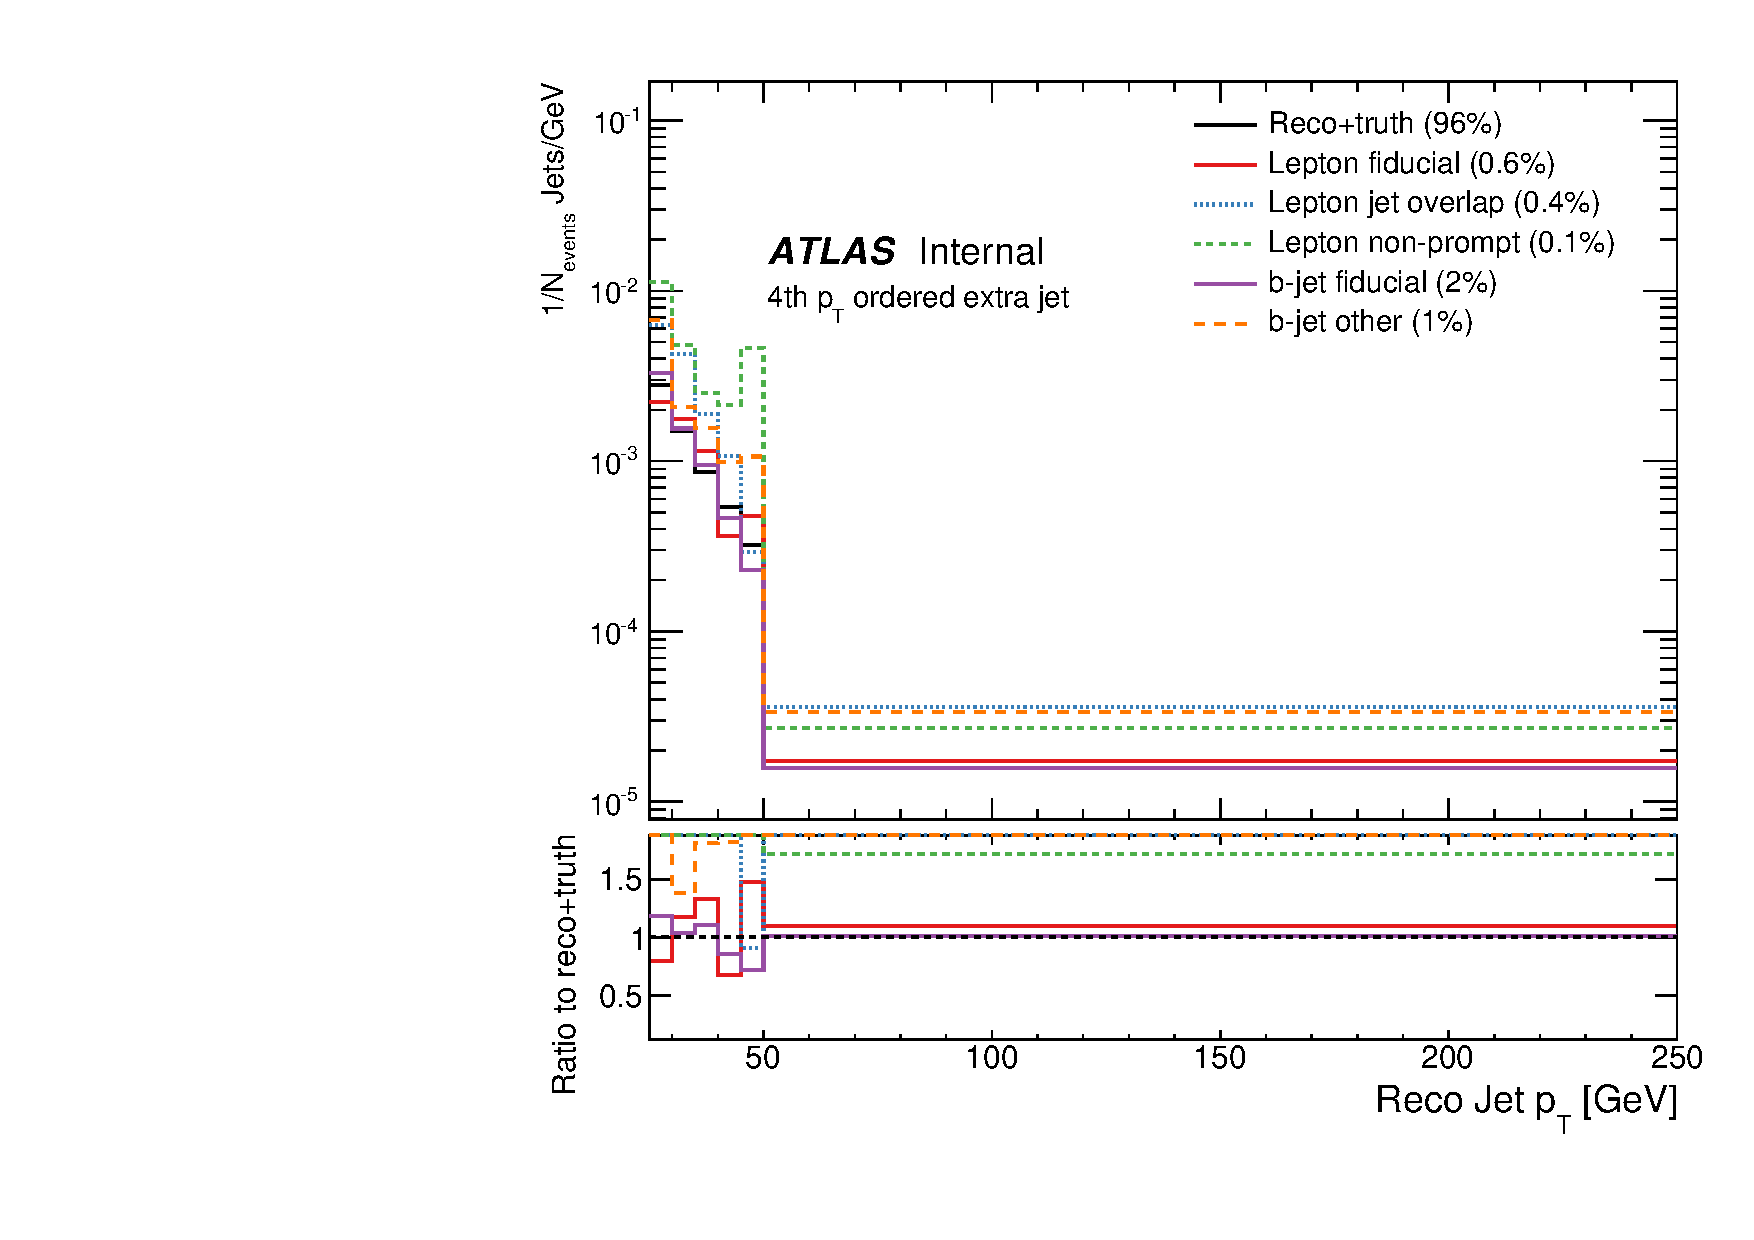
\includegraphics[width=\textwidth]{fig/RecoNotTruth/RecoPtJet3.pdf}
\end{subfigure}
~
\begin{subfigure}[]{0.3\textwidth}
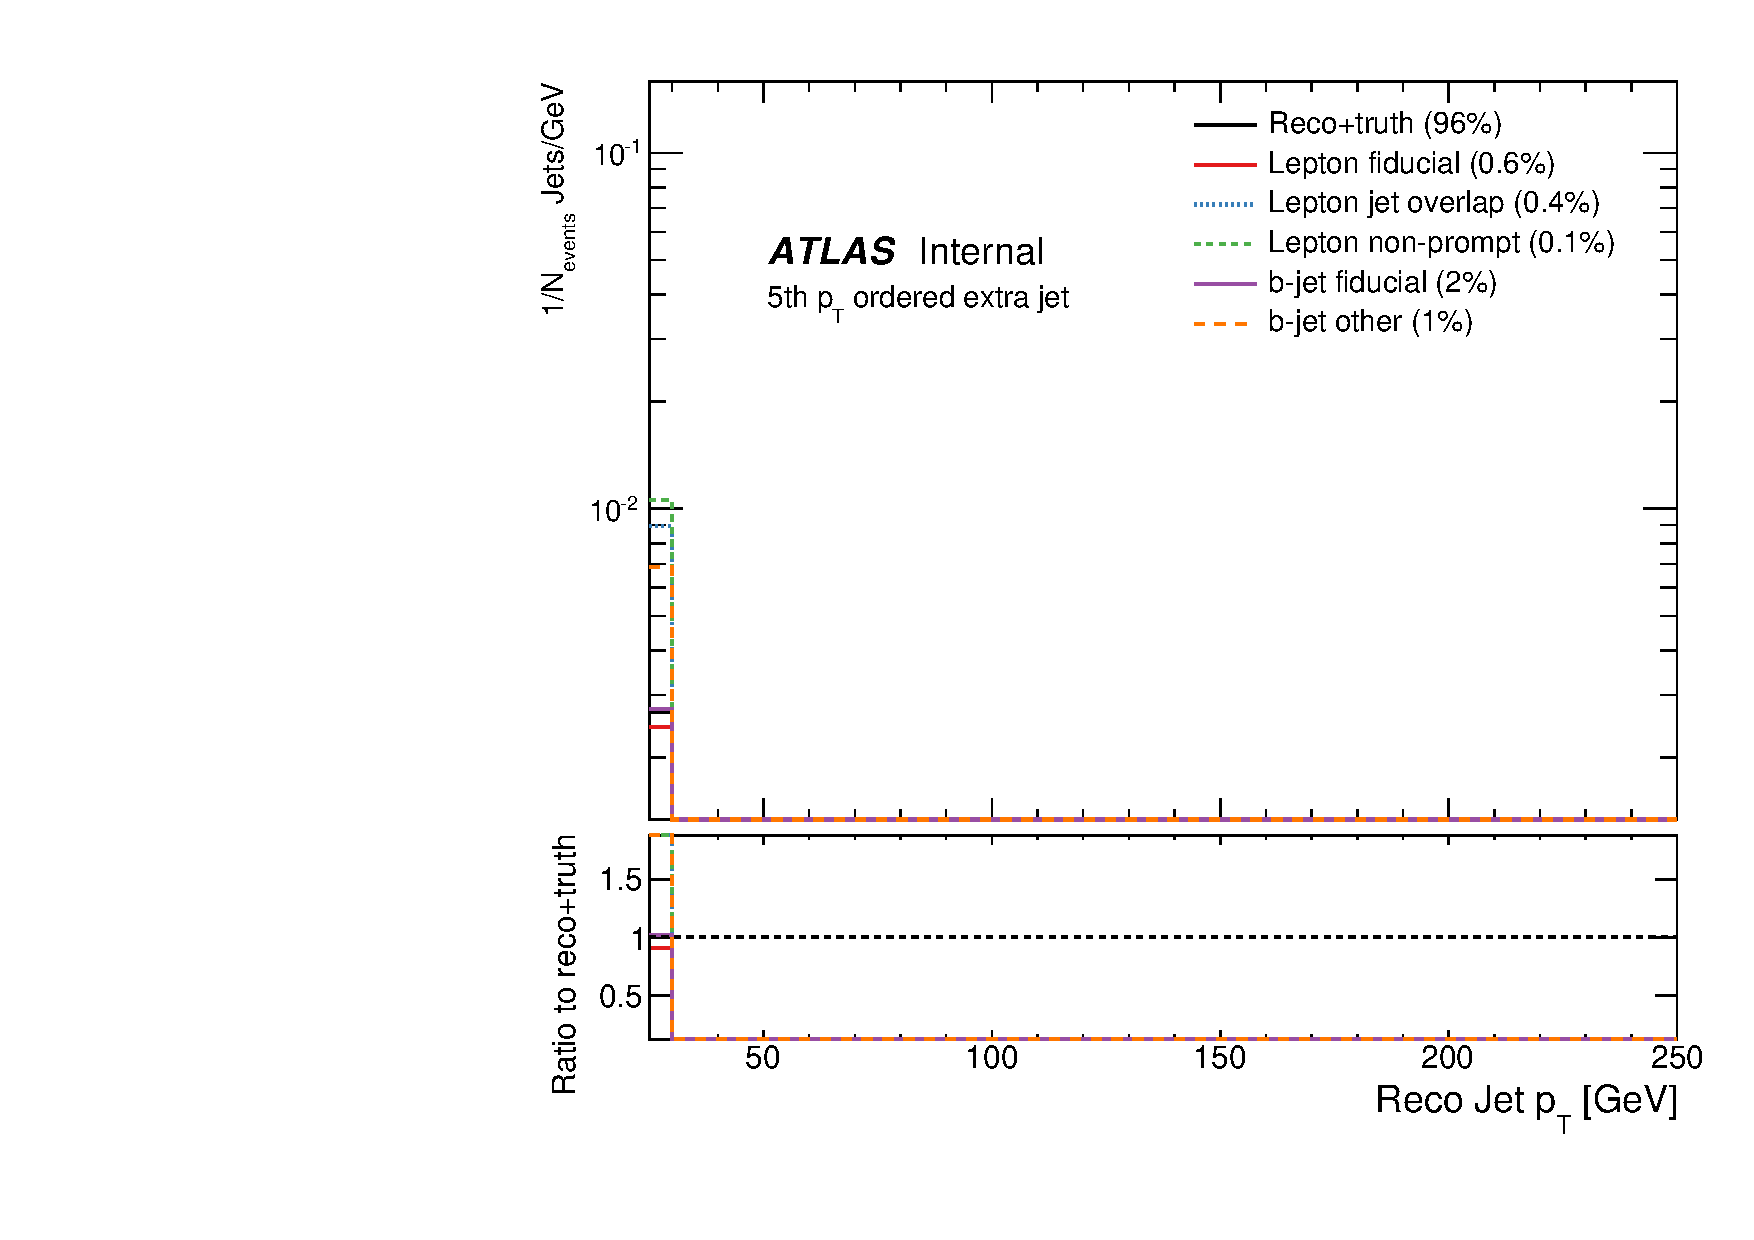
\includegraphics[width=\textwidth]{fig/RecoNotTruth/RecoPtJet4.pdf}
\end{subfigure}

\caption{Distributions of the reconstructed extra jet multiplicty and extra jet \pt for events in different truth categories. Each distribution is normalized by the number of events falling in that category. }
\label{fig:fakejetpt}

\end{figure}

\clearpage
